\documentclass{article}

\setcounter{secnumdepth}{0}

% Allow UTF-8 input
\usepackage[utf8]{inputenc} % allow utf-8 input
% Use 8-bit T1 fonts
\usepackage[T1]{fontenc}    

% Margins
\usepackage{geometry}
 \geometry{
  a4paper,
  left=25mm,
  top=25mm,
  right=25mm,
  left=25mm
 }
 
% Images
\usepackage{float}
\usepackage{graphicx}
\usepackage{subcaption}

% Item Enumeration
\usepackage{enumitem}
% Easy List
\usepackage[ampersand]{easylist}

% References
\usepackage{hyperref}

\title{Identificación y Control Neuronal}

\author{
  Pablo Acereda García\\
  Department of Computer Science\\
  University of Alcala\\
  28805 - Alcalá de Henares, Madrid, Spain \\
  \texttt{pablo.acereda@edu.uah.es} \\
  %% examples of more authors
   \And
  Laura Pérez Medeiro\\
  Department of Computer Science\\
  University of Alcala\\
  28805 - Alcalá de Henares, Madrid, Spain \\
  \texttt{l.perezm@edu.uah.es} \\
  %% \AND
  %% Coauthor \\
  %% Affiliation \\
  %% Address \\
  %% \texttt{email} \\
  %% \And
  %% Coauthor \\
  %% Affiliation \\
  %% Address \\
  %% \texttt{email} \\
  %% \And
  %% Coauthor \\
  %% Affiliation \\
  %% Address \\
  %% \texttt{email} \\
}

\begin{document}

% Title
\maketitle

% This page has been left blank intentionally
\newpage
\vspace*{\fill}
 \begin{center}
This page has been intentionally left blank
 \end{center}
\vspace*{\fill}
\newpage

% Table of contents
\tableofcontents

\newpage

\section{Ejercicio 1. Perceptron}

El Perceptron es una función de tipo lineal, que puede resultar indicada cuando
solo hay 2 clases dentro del conjunto de datos. Por este mismo motivo, este tipo
de red neuronal no es perfectamente funcional cuando hay diferentes clases (en
este caso 4).

Debido a que no se ha definido con anterioridad a la creación de la red
neuronal, el número de neuronas de la capa de salida es una (al igual que el
número de capas y el número de entradas).

\begin{figure}[H]
 \centering
 \begin{subfigure}{0.45\textwidth}
  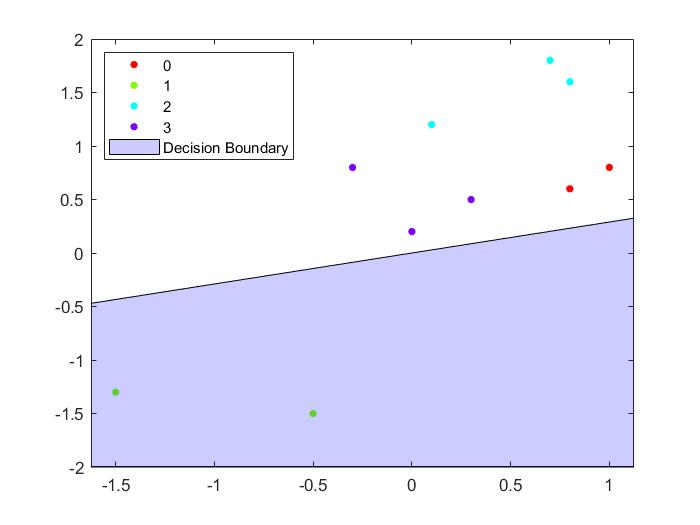
\includegraphics[width=0.9\linewidth]{../images/I_ex1_basicData.jpg}
  \caption{Datos Originales}
  \label{bs}
 \end{subfigure}
 \begin{subfigure}{0.45\textwidth}
  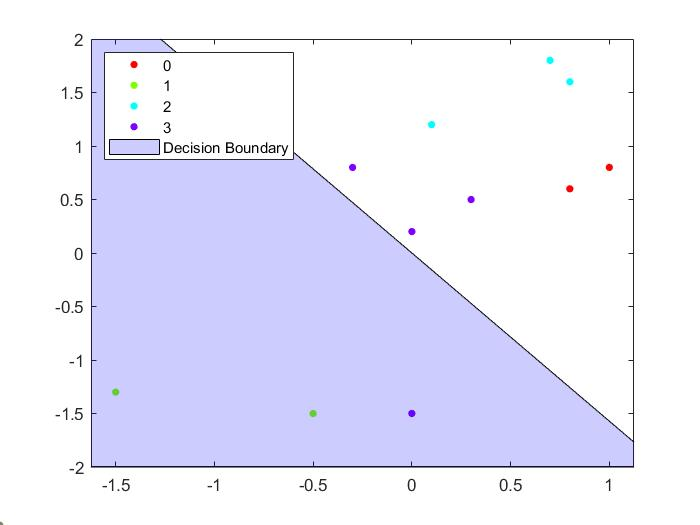
\includegraphics[width=0.9\linewidth]{../images/I_ex1_extendedData.jpg}
  \caption{Datos Extendidos}
  \label{ed}
 \end{subfigure}
\end{figure}

En la gráfica \hyperref[bs]{\ref{bs}} la pendiente obtenida por el perceptrón
separa los elementos de la clase \textit{1} del resto de elementos. Pero al
añadir el dato \texttt{$\left[0.0, -1.5\right]$} de la clase \textit{3}, el perceptrón
obtenido cambia completamente su pendiente (llegando incluso a invertirla). Con
la nueva pendiente es incapaz de separar completamente la clase \textit{1} de la
clase \textit{3}. Resultado a esperarse debido a que hay más clases y más
\textit{clusters} de los que puede separar un perceptrón\footnote{Xor Problem.}.

\section{Ejercicio 2. Aproximación de funciones}

La función sobre la que se quiere experimentar es $\sin(t)$. Se desea comprobar
si el modificar el número de neuronas de la capa ocula o cambiar el método de
entrenamiento posee algún efecto sobre un conjunto de datos.

En primera instancia, se ejecuta el \textit{script} con el método de
entrenamiento \textit{trainrp}, modificando el número de neuronas de la capa
oculta. Para las pruebas, se han empleado valores desde 3 hasta 5.

\begin{figure}[H]
 \centering
 \begin{subfigure}{0.3\textwidth}
  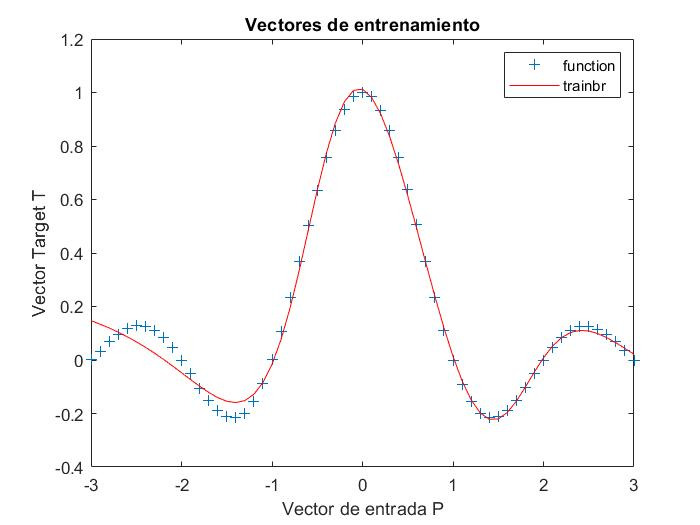
\includegraphics[width=0.8\linewidth]{../images/I_ex2_trainbr_3.jpg}
  \caption{\textit{trainbr}. Número neuronas de la capa oculta = 3.}
 \end{subfigure}
 \begin{subfigure}{0.3\textwidth}
  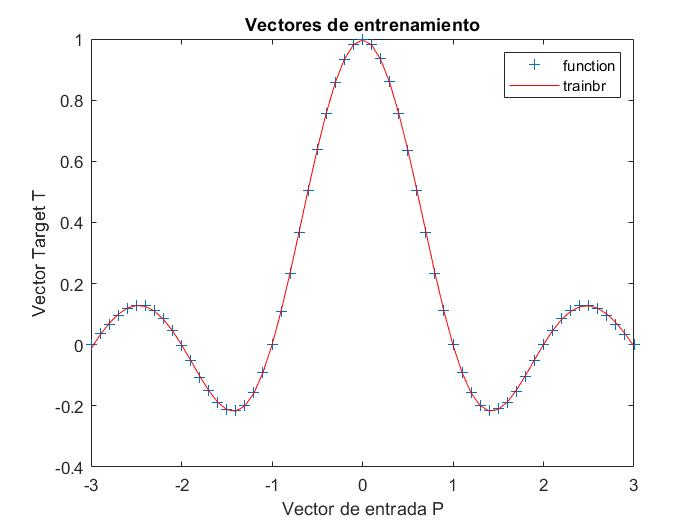
\includegraphics[width=0.8\linewidth]{../images/I_ex2_trainbr_4.jpg}
  \caption{\textit{trainbr}. Número neuronas de la capa oculta = 4.}
 \end{subfigure}
 \begin{subfigure}{0.3\textwidth}
  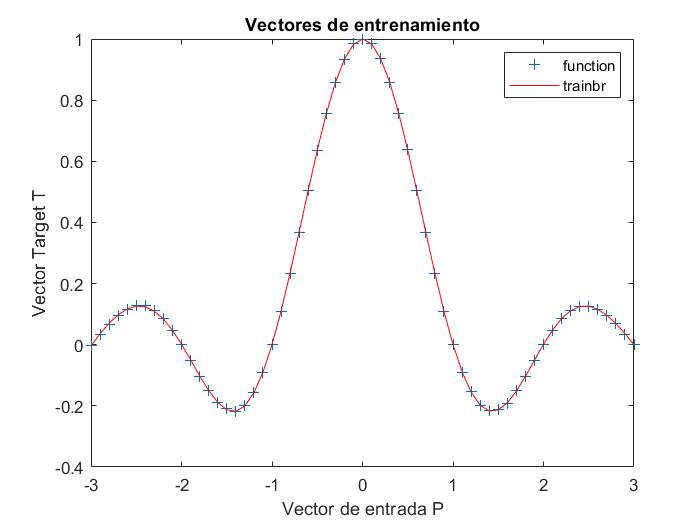
\includegraphics[width=0.8\linewidth]{../images/I_ex2_trainbr_5.jpg}
  \caption{\textit{trainbr}. Número neuronas de la capa oculta = 5.}
 \end{subfigure}
\end{figure}

Se comprobará en la figura \hyperref[f200]{\ref{f200}} como puede afectar el
número de neuronas de la capa oculta conforme aumenta su tamaño.

Además de modificar el número de neuronas de la capa oculta también se ha
modificado el método de entrenamiento, empleándose los siguientes:

\begin{description}
 \item [trainbr] Bayesan Regularization
 \item [trainrp] Resilient Backpropagation
 \item [trainoss] One Step Secant
 \item [traingd] Gradient Descent
\end{description}

El resultado se puede observar en las siguientes gráficas
(\hyperref[f4]{\ref{f4}} y \hyperref[f200]{\ref{f200}}).

\begin{figure}
 \centering
 \begin{subfigure}{0.45\textwidth}
  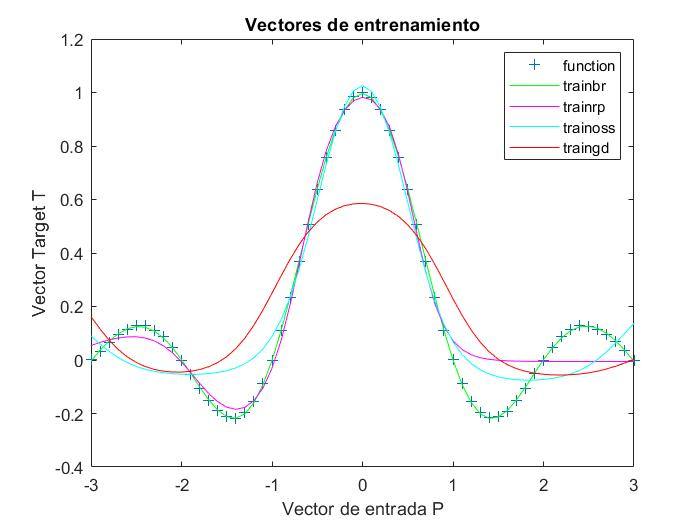
\includegraphics[width=0.9\linewidth]{../images/I_ex2_training_functions.jpg}
  \caption{Todas las funciones. Número de neuronas de la capa oculta = 4.}
  \label{f4}
 \end{subfigure}
 \begin{subfigure}{0.45\textwidth}
  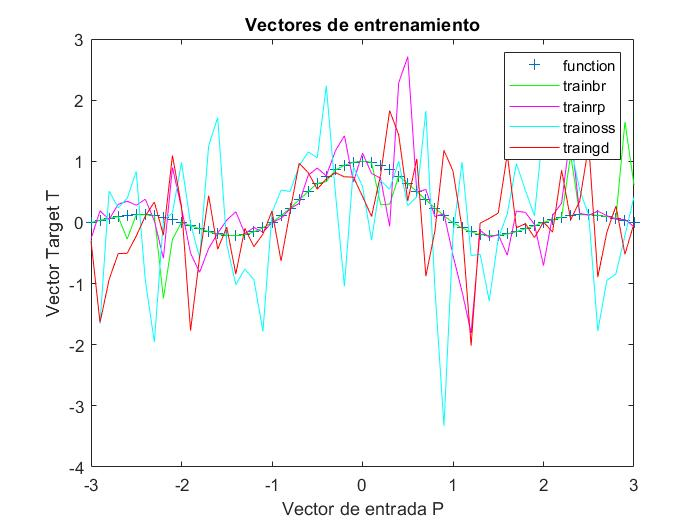
\includegraphics[width=0.9\linewidth]{../images/I_ex2_training_functions_200.jpg}
  \caption{Todas las funciones. Número de neuronas de la capa oculta = 200.}
  \label{f200}
 \end{subfigure}
\end{figure}

El modificar el número de neuronas de la capa oculta puede acabar en una red
neuronal que esté demasiado adaptada al problema, y que por lo tanto no tenga un
buen rendimiento al comprobar nuevos datos.

Además, el cambiar el método de entrenamiento supone el tener aproximaciones
diferentes. El elegir un método u otro siempre dependerá de la función original
o del conjunto de datos con los que se desea entrenar la red neuronal.

\section{Ejercicio 3. Aproximación de funciones (II)}

Tras la ejecución del algoritmo proporcionado y aplicarlo a
\textit{bodfat\textunderscore dataset} se obtienen las siguientes gráficas: 

\begin{figure}[H]
 \centering
 \begin{subfigure}{0.4\textwidth}
  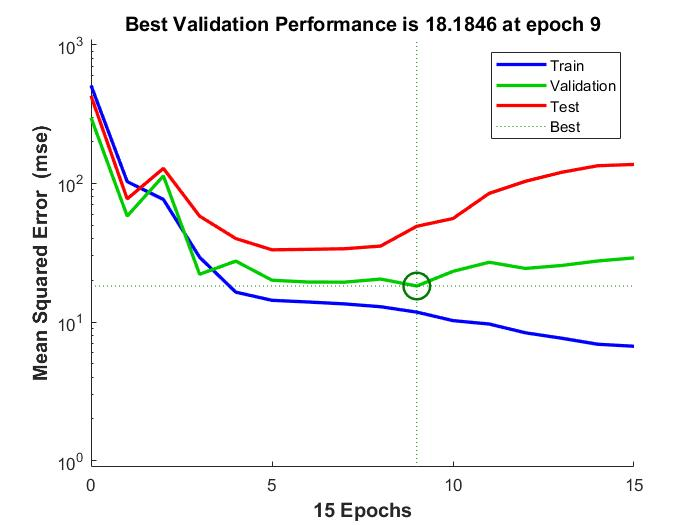
\includegraphics[width=0.8\linewidth]{../images/I_ex3_performance_bodyfat_dataset.jpg}
  \caption{Rendimiento}
 \end{subfigure}
 \begin{subfigure}{0.4\textwidth}
  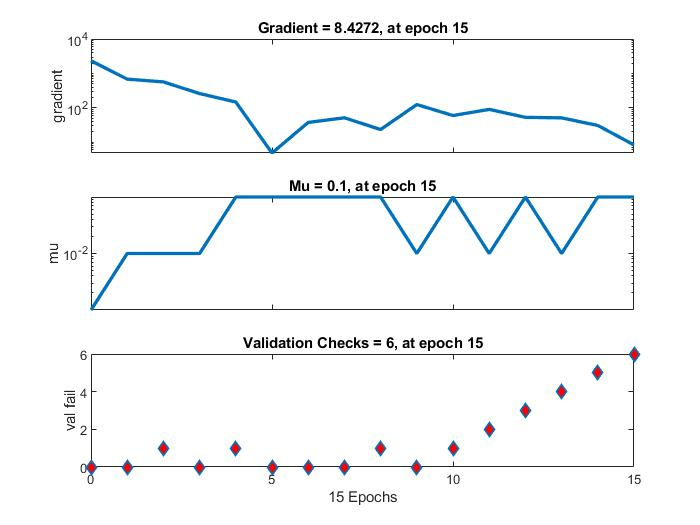
\includegraphics[width=0.8\linewidth]{../images/I_ex3_trainingstate_bodyfat_dataset.jpg}
  \caption{Estado de Entrenamiento}
 \end{subfigure}
 \begin{subfigure}{0.4\textwidth}
  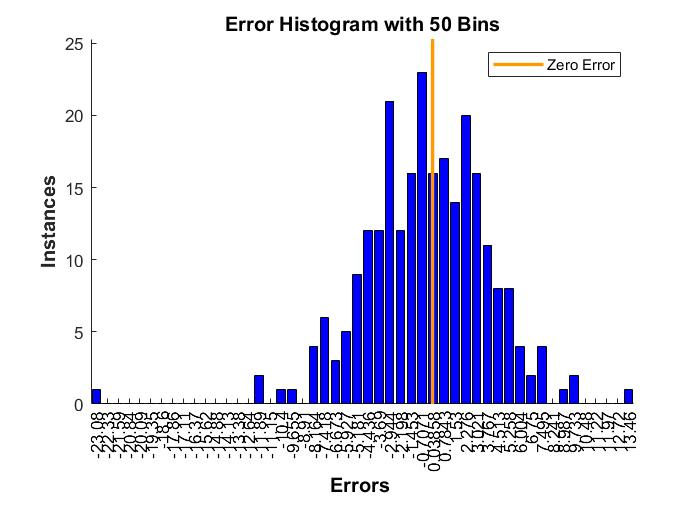
\includegraphics[width=0.8\linewidth]{../images/I_ex3_errorhistogram_bodyfat_dataset.jpg}
  \caption{Histograma de Errores}
 \end{subfigure}
 \begin{subfigure}{0.4\textwidth}
  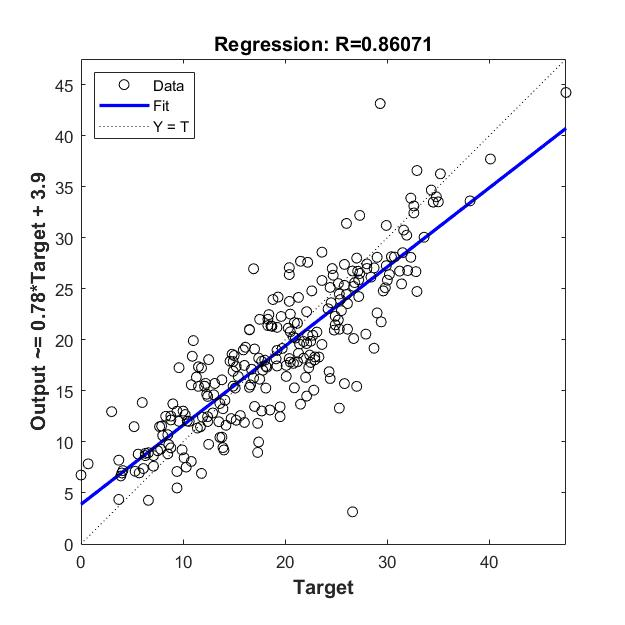
\includegraphics[width=0.8\linewidth]{../images/I_ex3_regression_bodyfat_dataset.jpg}
  \caption{Regresión}
 \end{subfigure}
\end{figure}

Los resultados demuestran que el entrenamiento de la red neuronal aumenta en
precisión conforme avanzan las épocas (\textit{epoch}); la validación encuentra
su error mínimo durante el periodo 9, momento a partir del cual solo aumenta; en
el testing, el error aumenta tras durante el testeo, llegado a alcanzar más de 
$10^2$ (un valor demasiado alto).

Para solucionar este problema, se puede probar una distribución de los datos
diferente. En este caso se ha escogido 60/20/20 como valores para el
entrenamiento (\textit{train}), la validación (\textit{validation}) y el testeo
(\textit{test}), respectivamente, de manera arbitraria.

\begin{figure}[H]
 \centering
 \begin{subfigure}{0.4\textwidth}
  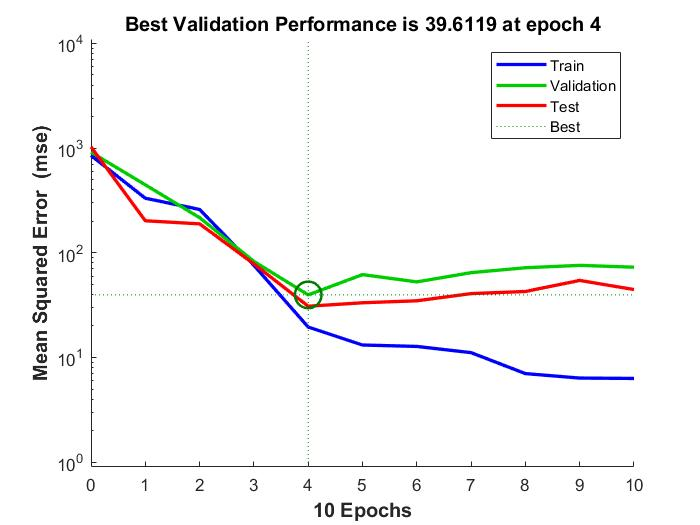
\includegraphics[width=0.8\linewidth]{../images/I_ex3_performance_bodyfat_dataset_div60-20-20.jpg}
  \caption{Rendimiento}
 \end{subfigure}
 \begin{subfigure}{0.4\textwidth}
  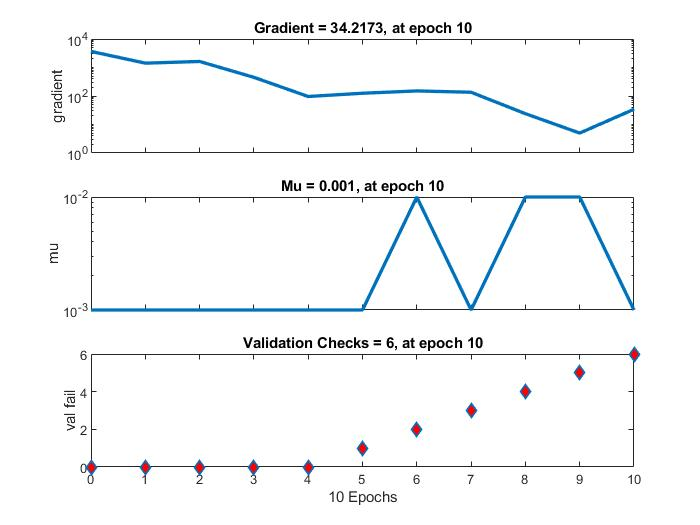
\includegraphics[width=0.8\linewidth]{../images/I_ex3_trainingstate_bodyfat_dataset_div60-20-20.jpg}
  \caption{Estado de Entrenamiento}
 \end{subfigure}
 \begin{subfigure}{0.4\textwidth}
  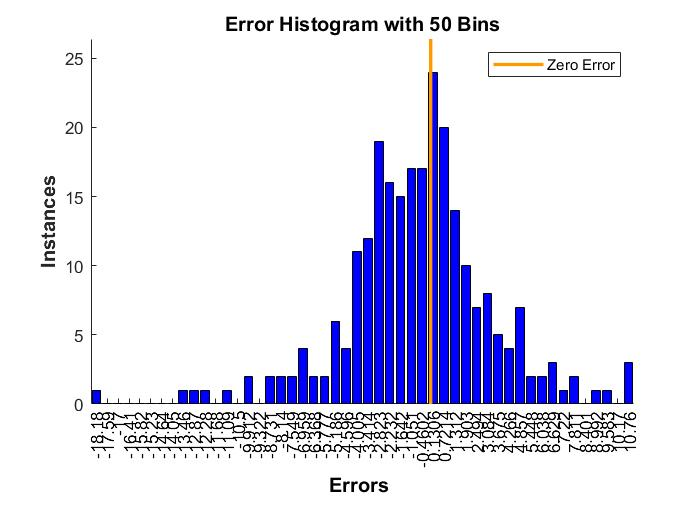
\includegraphics[width=0.8\linewidth]{../images/I_ex3_errorhistogram_bodyfat_dataset_div60-20-20.jpg}
  \caption{Histograma de Errores}
 \end{subfigure}
 \begin{subfigure}{0.4\textwidth}
  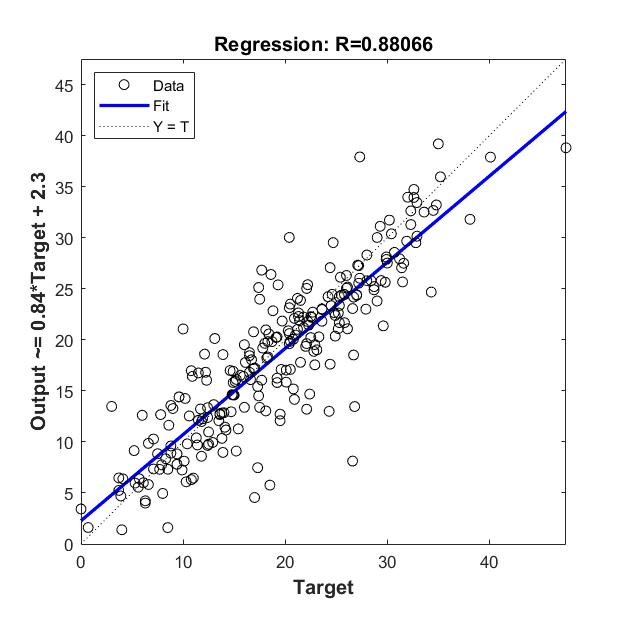
\includegraphics[width=0.8\linewidth]{../images/I_ex3_regression_bodyfat_dataset_div60-20-20.jpg}
  \caption{Regresión}
 \end{subfigure}
\end{figure}

Tras la nueva división de los datos, empleando el mismo algoritmo de
entrenamiento, se consigue que los errores (teste, validación y entrenamiento)
disminuyen, aunque la valicación y el test siguen teniendo una cierta
predisposición a incrementar levemente superada la cuarta época. 

La función lineal mostrada en la regresión pasa a ser de $Output ~= 0.78*Target
+ 3.9$ a valer $Output ~= 0.84*Target + 2.3$. Siendo, aparentemente, la segunda
una ecuación más fiel a los datos representados.

Para realizar un estudio más exhaustivo, se han empleado diferentes métodos de
entrenamiento.

\begin{description}
\item [trainbr] Bayesan Regularization
\item [trainrp] Resilient Backpropagation
\item [trainoss] One Step Secant
\item [traingd] Gradient Descent
\end{description}

A continuación se especificará y comparará cada uno de los grupos de gráficas
obtenidos a lo largo de la ejecución del \textit{script}

Referente al rendimiento, la función bayesiana ha conseguido los mejores
resultados, consigue el mejor rendimiento de entre las cuatro gráficas. Por otro
lado, la función \textit{trainrp} consigue un rendimiento que empeora conforme
se supera la época 16. \textit{trainoss}, con un rendimiento entre las dos
anteriores, posee un MSE muy similar entre los conjuntos de datos
\textit{train}, \textit{validation} y \textit{test}. Por último, el método de
entrenamiento del gradicente, consigue el peor resultado, empeorando conforme
recibe más entrenamiento.

\begin{figure}[H]
 \centering
 \begin{subfigure}{0.4\textwidth}
  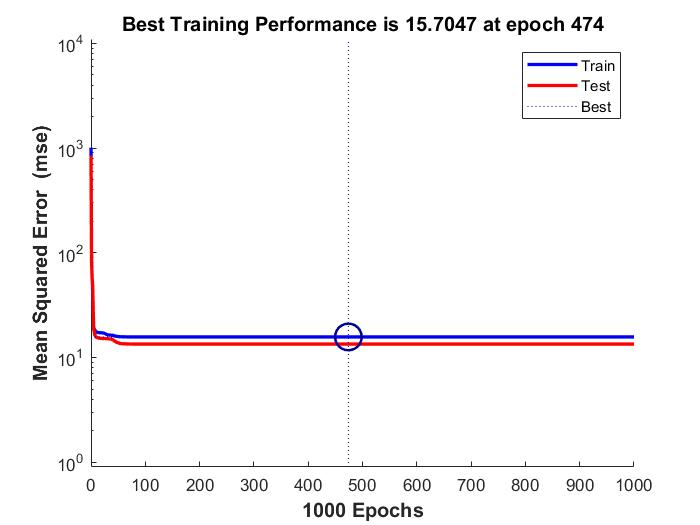
\includegraphics[width=0.8\linewidth]{../images/I_ex3_performance_bodyfat_dataset_trainbr.jpg}
  \caption{Rendimiento \textit{trainbr}}
 \end{subfigure}
 \begin{subfigure}{0.4\textwidth}
  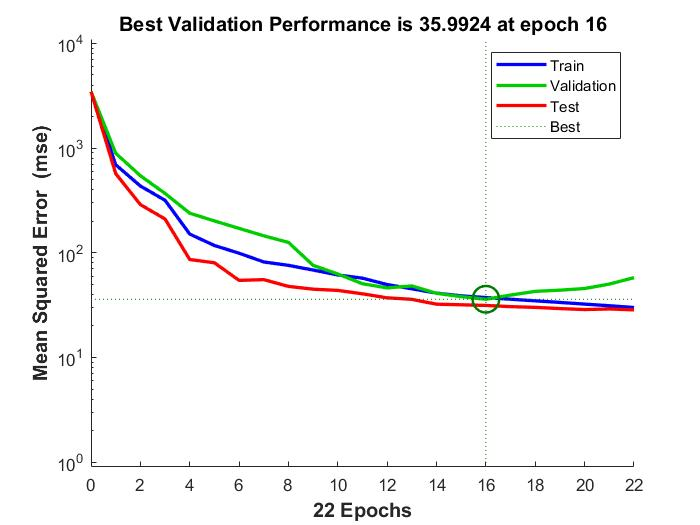
\includegraphics[width=0.8\linewidth]{../images/I_ex3_performance_bodyfat_dataset_trainrp.jpg}
  \caption{Rendimiento \textit{trainrp}}
 \end{subfigure}
 \begin{subfigure}{0.4\textwidth}
  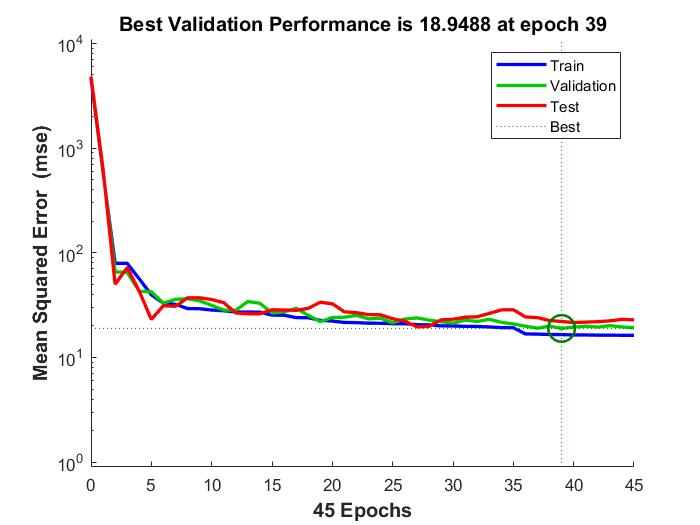
\includegraphics[width=0.8\linewidth]{../images/I_ex3_performance_bodyfat_dataset_trainoss.jpg}
  \caption{Rendimiento \textit{trainoss}}
 \end{subfigure}
 \begin{subfigure}{0.4\textwidth}
  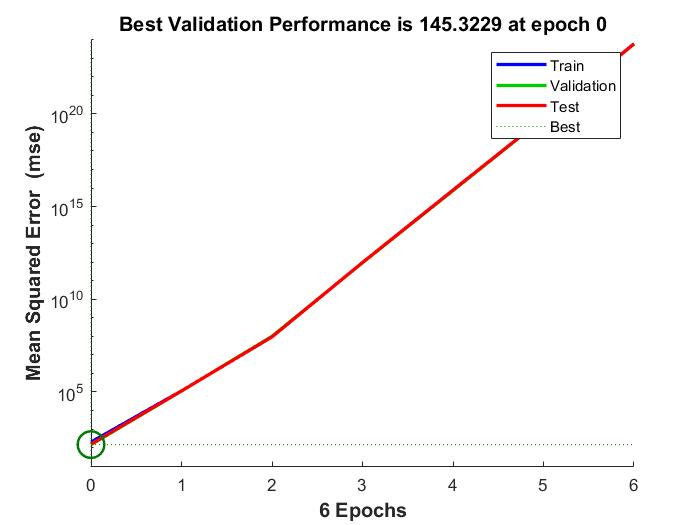
\includegraphics[width=0.8\linewidth]{../images/I_ex3_performance_bodyfat_dataset_traingd.jpg}
  \caption{Rendimiento \textit{traingd}}
 \end{subfigure}
\end{figure}

El valor del gradiente \footnote{El valor del gradiente por propagación inversa
se encuentra en escala logarítmica. El valor en la parte superior de la gráfica
es el valor para el cual se ha alcanzado el punto mínimo de un mínimo local.} se 
muestra una vez más incremental para \textit{traingd}\footnote{MATLAB detiene el 
entrenamiento del modelo cuando el valor de MSE - Mean Square Error - resulta 
incremental 6 veces de manera consecutiva, también conocido como 
\textit{validation fails}.} En el caso de \textit{trainbr}, el gradiente se 
mantiene constante a partir de cierto punto, lo que hace que el entrenamiento 
dure 1000 \textit{epochs}; esto se debe a la manera en la que está codificado el
algoritmo, la parada por valiación se encuentra desactivada por defecto. El 
entrenamiento de \textit{trainrp} y \textit{trainoss} discurre de manera normal, 
alcanzando los mínimos locales en los valores 11.2225 y 39.6971, respectivamente.

\begin{figure}[H]
\centering
 \begin{subfigure}{0.4\textwidth}
  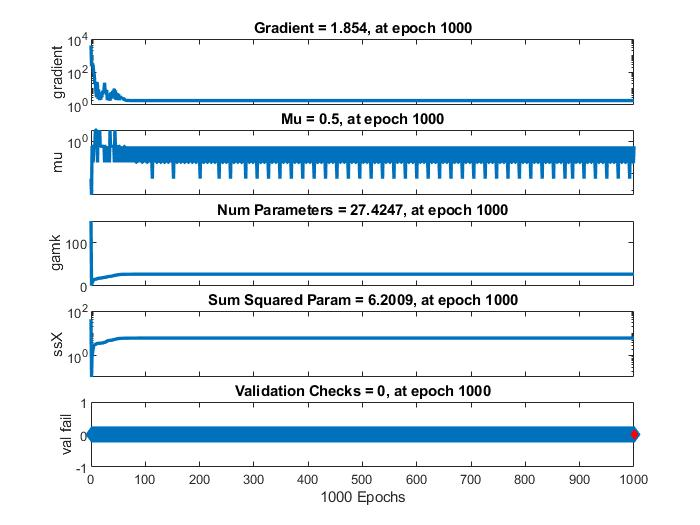
\includegraphics[width=0.8\linewidth]{../images/I_ex3_trainingstate_bodyfat_dataset_trainbr.jpg}
  \caption{Estado de Entrenamiento \textit{trainbr}}
 \end{subfigure}
 \begin{subfigure}{0.4\textwidth}
  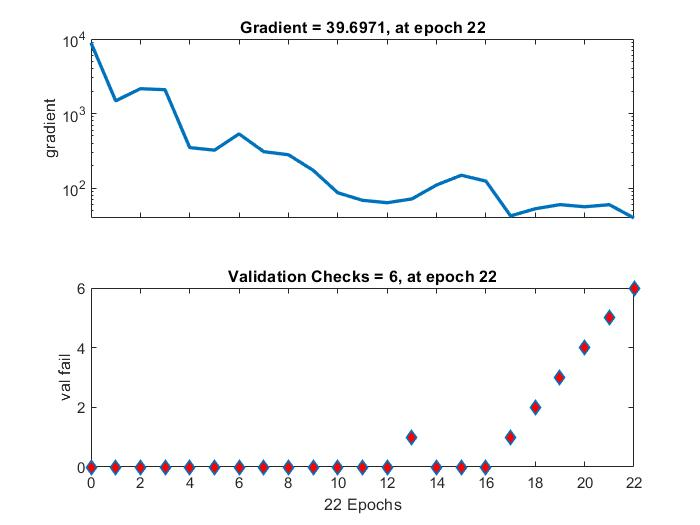
\includegraphics[width=0.8\linewidth]{../images/I_ex3_trainingstate_bodyfat_dataset_trainrp.jpg}
  \caption{Estado de Entrenamiento \textit{trainrp}}
 \end{subfigure}
 \begin{subfigure}{0.4\textwidth}
  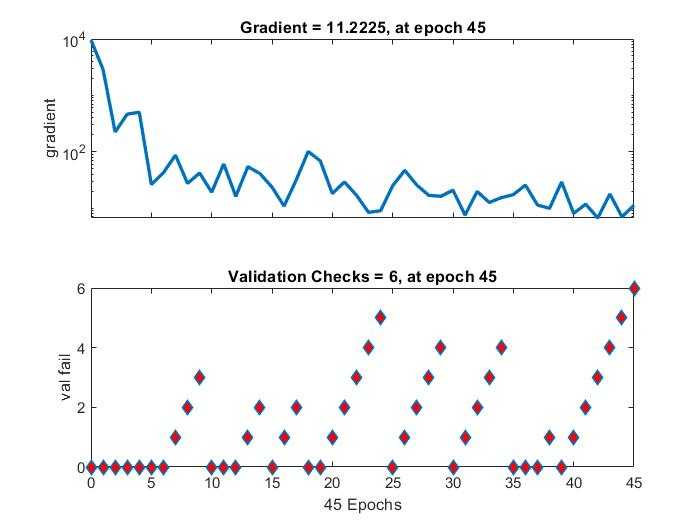
\includegraphics[width=0.8\linewidth]{../images/I_ex3_trainingstate_bodyfat_dataset_trainoss.jpg}
  \caption{Estado de Entrenamiento \textit{trainoss}}
 \end{subfigure}
 \begin{subfigure}{0.4\textwidth}
  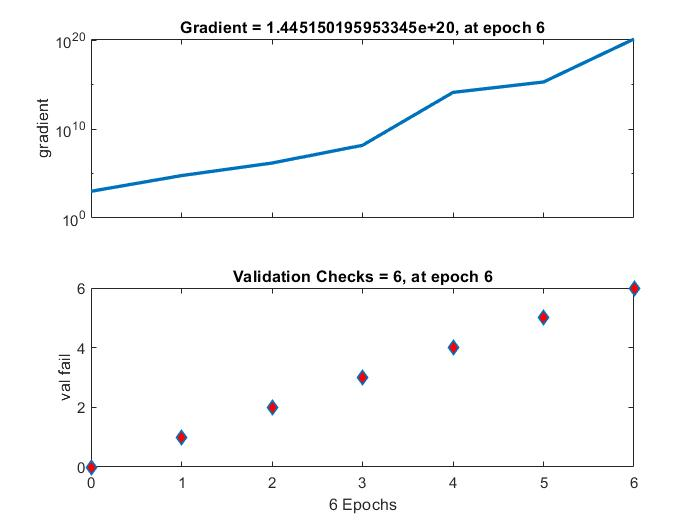
\includegraphics[width=0.8\linewidth]{../images/I_ex3_trainingstate_bodyfat_dataset_traingd.jpg}
  \caption{Estado de Entrenamiento \textit{traingd}}
 \end{subfigure}
\end{figure}

El histograma es una gráfica que representa el error cometido al estimar los
valores empleados para el entrenamiento de la red neuronal, por tanto, cuanto
más esté centrada la distribución de lo errores de manera cercana al indicador
\textit{Zero Error}, mejor predicción dará el modelo. Atendiendo a este
criterio, los extremos de \textit{trainrp} están prácticamente libres, y los
valores cercanos a $Error = 0$ están más poblados. Por esto mismo, se sabe que
la función del gradiente es la que ha obtenido peores resultados, por tener su
mayor concentración de errores más cercana a 1 que a 0. \textit{trainoss} tiene,
con alguna excepción, forma de pirámide escalonada, lo que también sugiere un
entrenamiento exitoso. \textit{trainbr} posee una forma bastante irregular, pero
los errores que más se repiten se encuentran principalmente en la zona central,
sugiriendo un resultado mejor que el resto de algoritmos de entrenamiento.

\begin{figure}[H]
 \centering
 \begin{subfigure}{0.4\textwidth}
  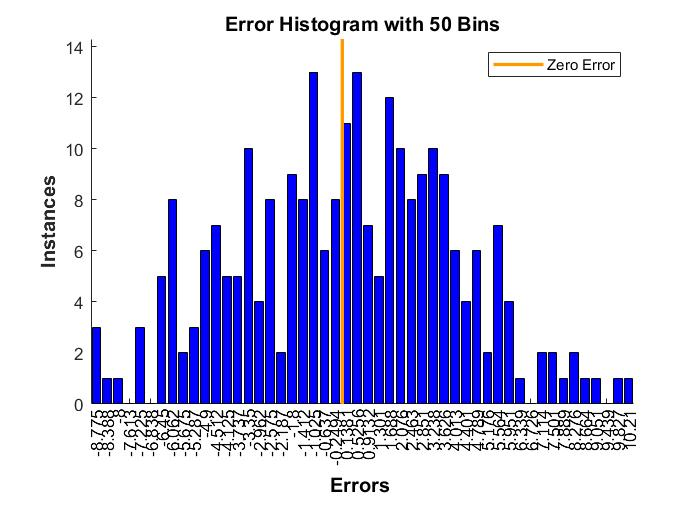
\includegraphics[width=0.8\linewidth]{../images/I_ex3_errorhistogram_bodyfat_dataset_trainbr.jpg}
  \caption{Histograma de Errores \textit{trainbr}}
 \end{subfigure}
 \begin{subfigure}{0.4\textwidth}
  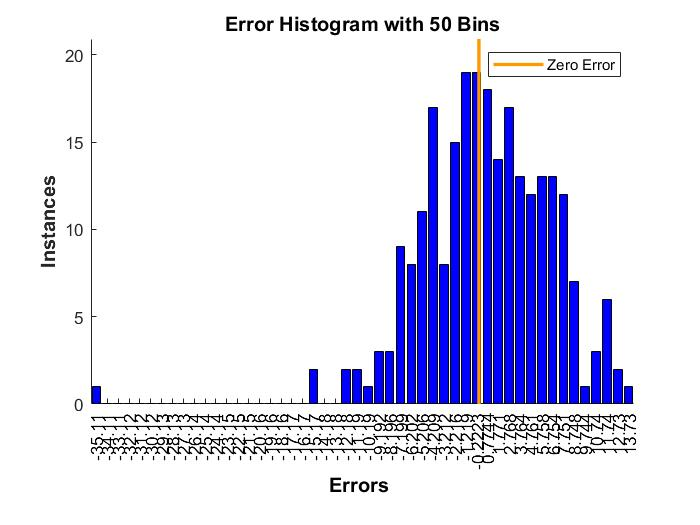
\includegraphics[width=0.8\linewidth]{../images/I_ex3_errorhistogram_bodyfat_dataset_trainrp.jpg}
  \caption{Histograma de Errores \textit{trainrp}}
 \end{subfigure}
 \begin{subfigure}{0.4\textwidth}
  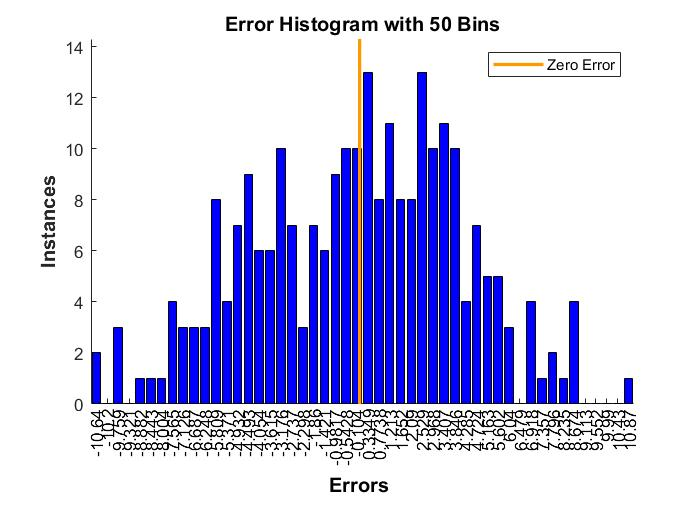
\includegraphics[width=0.8\linewidth]{../images/I_ex3_errorhistogram_bodyfat_dataset_trainoss.jpg}
  \caption{Histograma de Errores \textit{trainoss}}
 \end{subfigure}
 \begin{subfigure}{0.4\textwidth}
  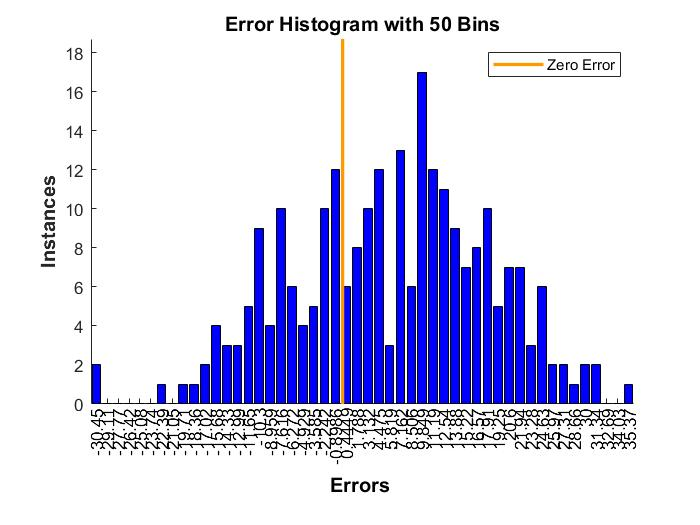
\includegraphics[width=0.8\linewidth]{../images/I_ex3_errorhistogram_bodyfat_dataset_traingd.jpg}
  \caption{Histograma de Errores \textit{traingd}}
 \end{subfigure}
\end{figure}
 
En la parte superior de cada gráfica aparece un valor, \textit{R}, el cual
indica lo óptima que es la regresión, siendo 1 el valor más óptimo. No hace
falta observar mucho los resultados obtenidos para percatarse de que el método
de entrenamiento más óptimo es en realidad la regularización bayesiana, tal y
como se venía adelantando a lo largo del ejercicio. 

\begin{figure}[H]
 \centering
 \begin{subfigure}{0.4\textwidth}
  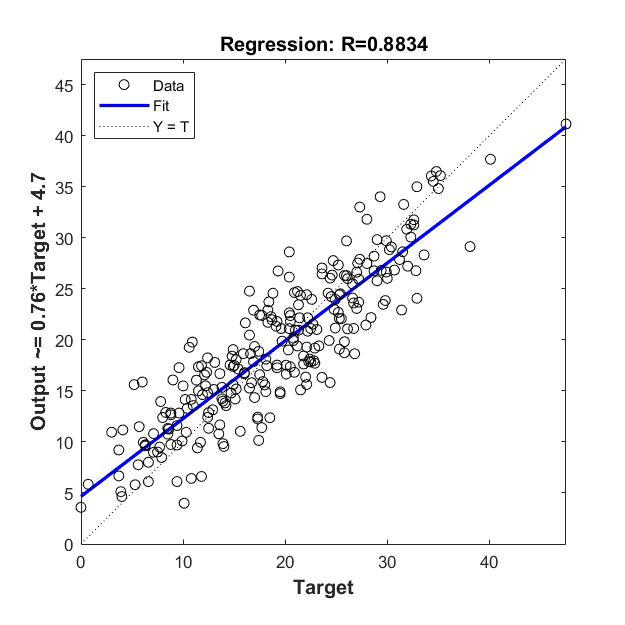
\includegraphics[width=0.8\linewidth]{../images/I_ex3_regression_bodyfat_dataset_trainbr.jpg}
  \caption{Regresión \textit{trainbr}}
 \end{subfigure}
 \begin{subfigure}{0.4\textwidth}
  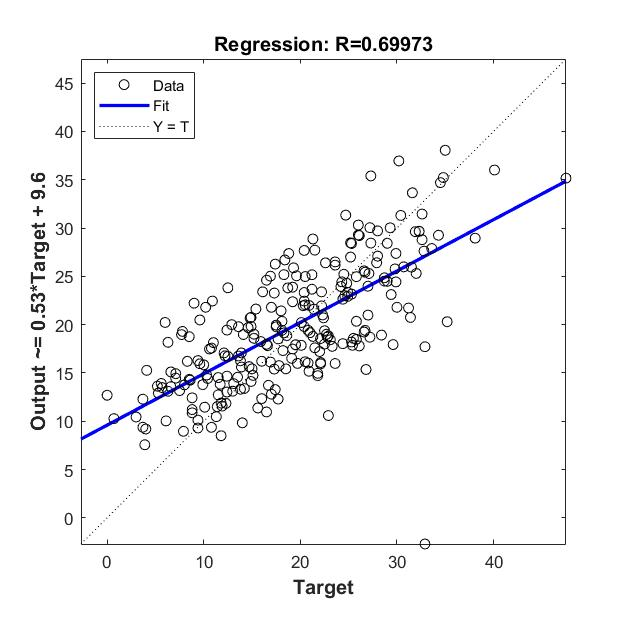
\includegraphics[width=0.8\linewidth]{../images/I_ex3_regression_bodyfat_dataset_trainrp.jpg}
  \caption{Regresión \textit{trainrp}}
 \end{subfigure}
 \begin{subfigure}{0.4\textwidth}
  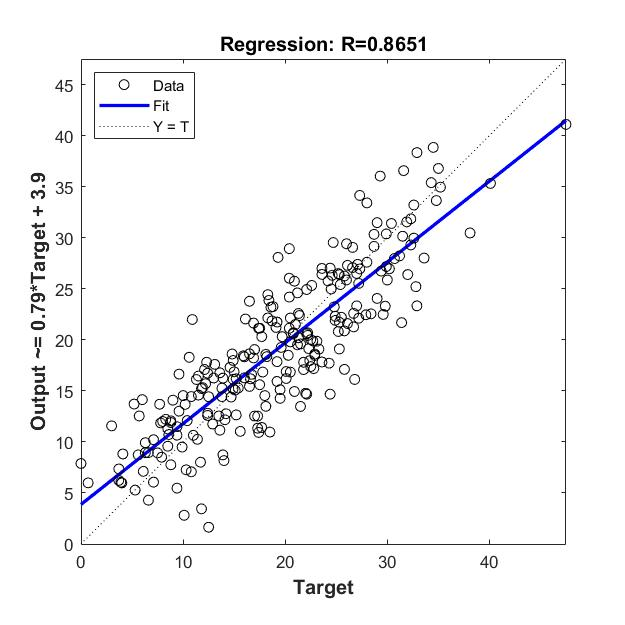
\includegraphics[width=0.8\linewidth]{../images/I_ex3_regression_bodyfat_dataset_trainoss.jpg}
  \caption{Regresión \textit{trainoss}}
 \end{subfigure}
 \begin{subfigure}{0.4\textwidth}
  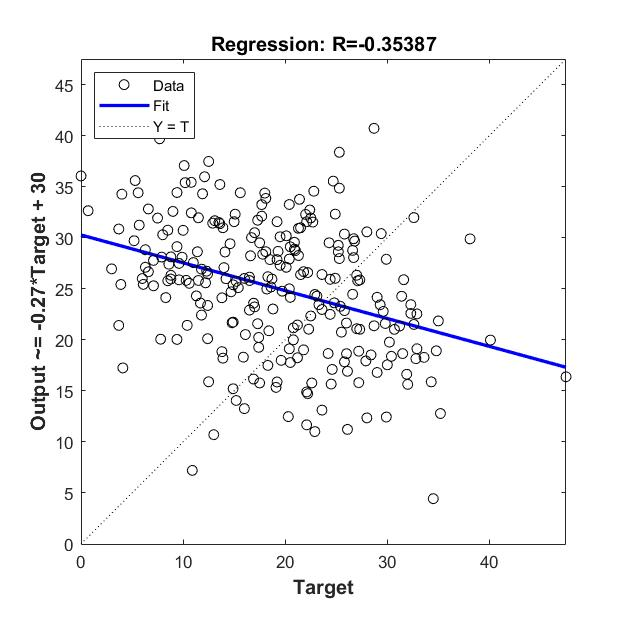
\includegraphics[width=0.8\linewidth]{../images/I_ex3_regression_bodyfat_dataset_traingd.jpg}
  \caption{Regresión \textit{traingd}}
 \end{subfigure}
\end{figure}

\section{Ejercicio 4. Clasificación}

Tras la ejecución del \textit{script} adaptado para los datos de
\textit{cancer\textunderscore dataset} se obtienen las siguientes gráficas.

\begin{figure}[H]
 \centering
 \begin{subfigure}{0.45\textwidth}
  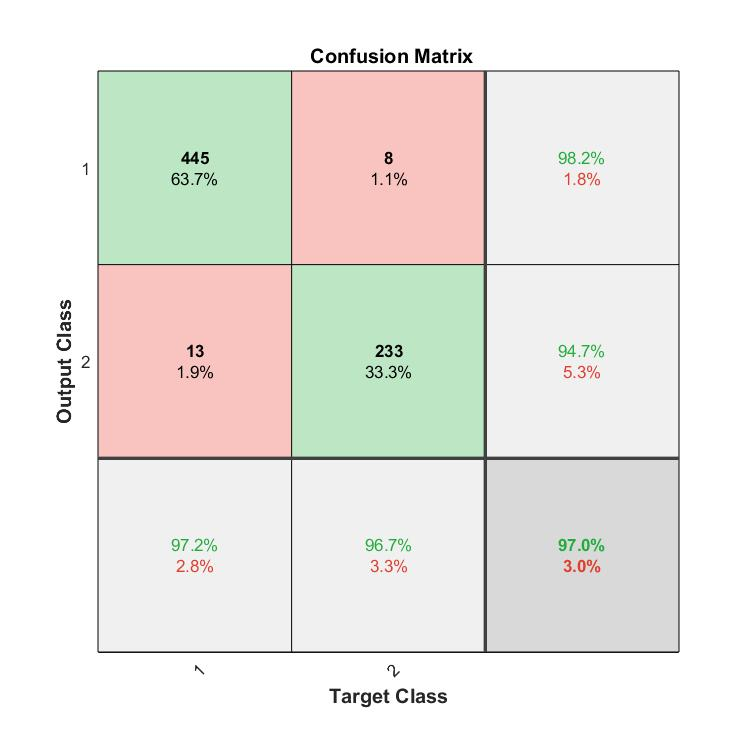
\includegraphics[width=0.9\linewidth]{../images/I_ex4_confusion_cancer_dataset.jpg}
  \caption{Matriz de confusión}
  \label{conf}
 \end{subfigure}
 \begin{subfigure}{0.45\textwidth}
  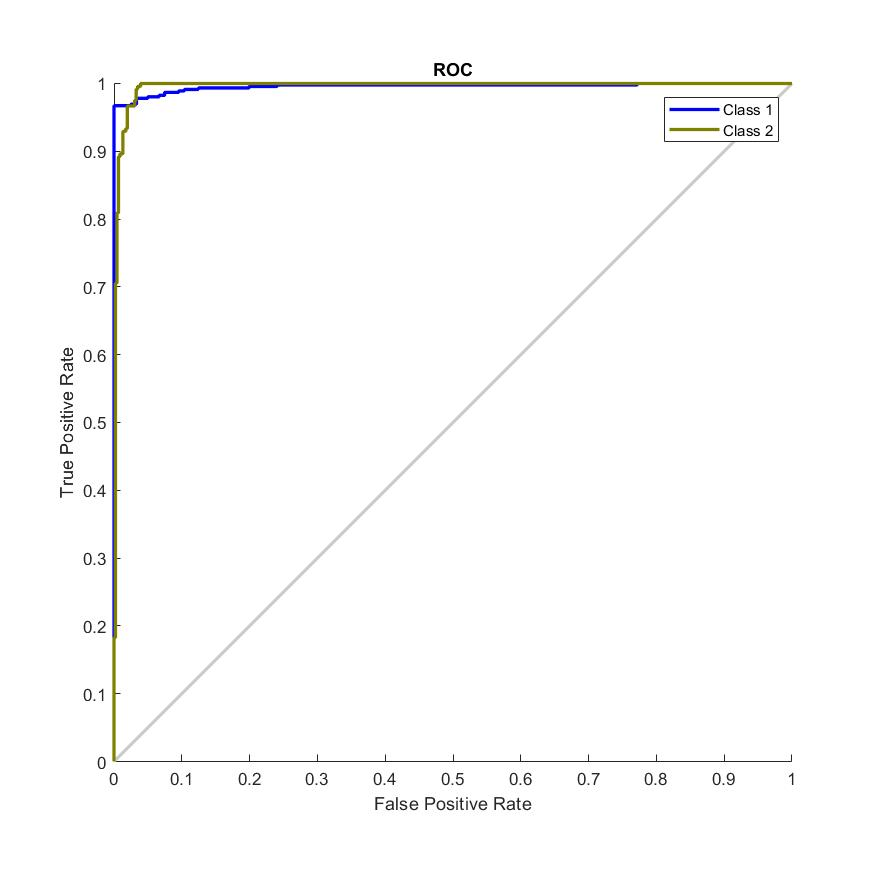
\includegraphics[width=0.9\linewidth]{../images/I_ex4_roc_cancer_dataset.jpg}
  \caption{\textit{Receiver Operating Characteristic}}
  \label{roc}
 \end{subfigure}
\end{figure}

En \hyperref[conf]{\ref{conf}}, las filas indican el valor que se ha predicho;
lsa columnas indican el valor real. Por tanto, la diagonal corresponde a los
valores que han sido predecidos de manera correcta. Interpretando el resultado
obtenido, se sabe que el 97\% de las estimaciones han sido correctas.

En la segunda gráfica (\hyperref[roc]{\ref{roc}}), es una métrica empleada para
comprobar la calidad de los clasificadores. Cuanto más se acerquen las funciones
a 1 en el eje de ordenadas. Por este mismo motivo, se conoce que los
clasificadores empleados para este set de datos son una buena opción.

Para realizar un estudio más acertado de estas herramientas, se han empleado
diferentes métods de entrenamiento (los mismos empleados para los ejercicios 2 y
3 de este mismo apartado).

\begin{figure}[H]
 \centering
 \begin{subfigure}{0.4\textwidth}
  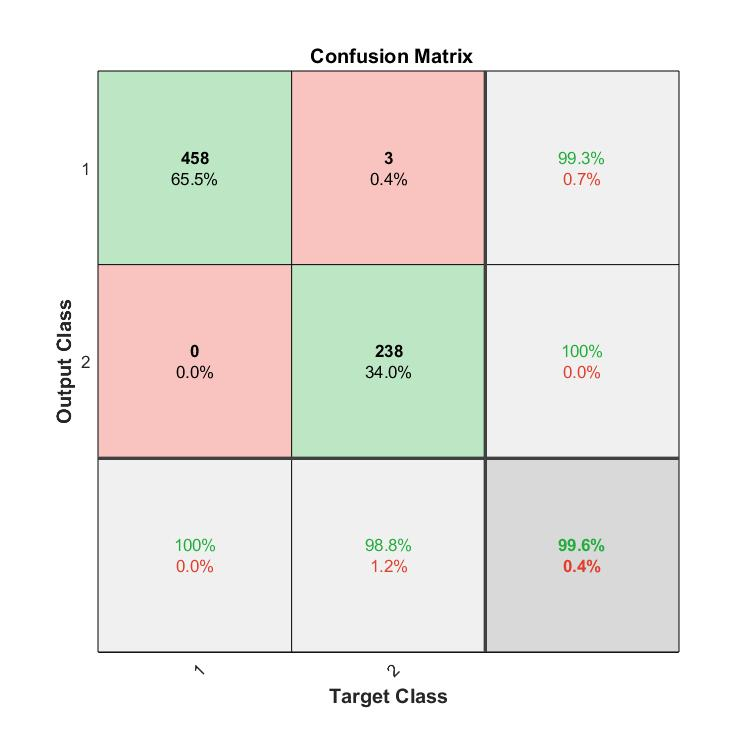
\includegraphics[width=0.8\linewidth]{../images/I_ex4_confusion_cancer_dataset_trainbr.jpg}
  \caption{Matriz de confusión \textit{trainbr}}
 \end{subfigure}
 \begin{subfigure}{0.4\textwidth}
  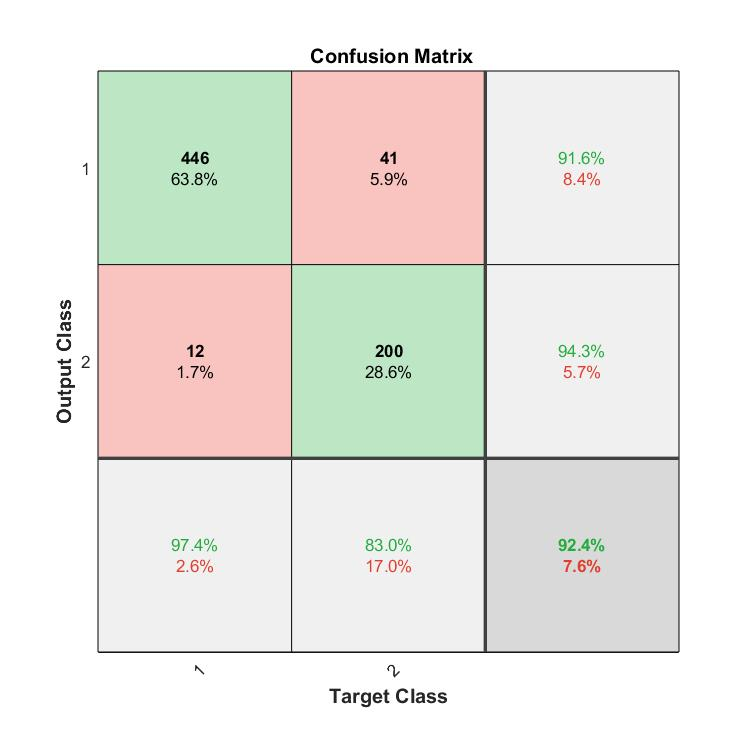
\includegraphics[width=0.8\linewidth]{../images/I_ex4_confusion_cancer_dataset_traingd.jpg}
  \caption{Matriz de confusión \textit{trainrp}}
 \end{subfigure}
 \begin{subfigure}{0.4\textwidth}
  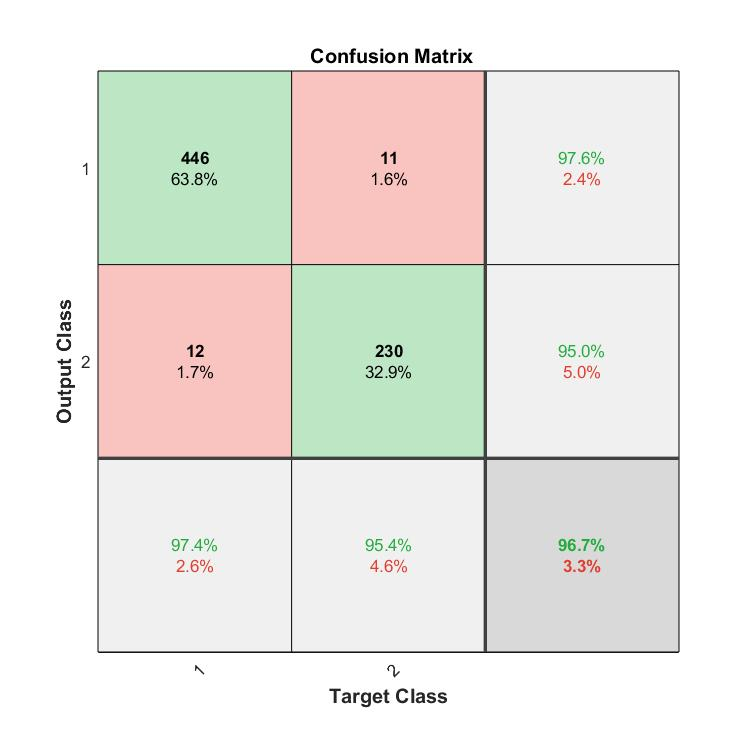
\includegraphics[width=0.8\linewidth]{../images/I_ex4_confusion_cancer_dataset_trainoss.jpg}
  \caption{Matriz de confusión \textit{trainoss}}
 \end{subfigure}
 \begin{subfigure}{0.4\textwidth}
  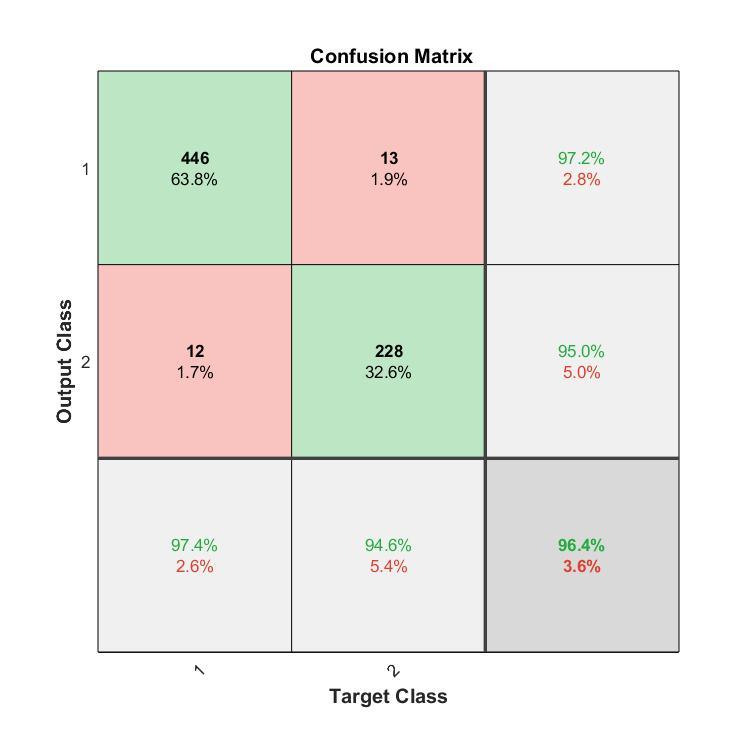
\includegraphics[width=0.8\linewidth]{../images/I_ex4_confusion_cancer_dataset_trainrp.jpg}  
  \caption{Matriz de confusión \textit{traingd}}
 \end{subfigure}
\end{figure}

De entre todos los resultados obtenidos, el más acertado ha sido el de el
algoritmo de entrenamiento \textit{trainbr}, con un 99.6\% de acierto sobre el
set. El peor algoritmo que se podría emplear sobre este set es \textit{trainrp},
que a pesar de poseer el peor resultado tiene un 92.4\% de acierto.

\begin{figure}[H]
 \centering
 \begin{subfigure}{0.4\textwidth}
  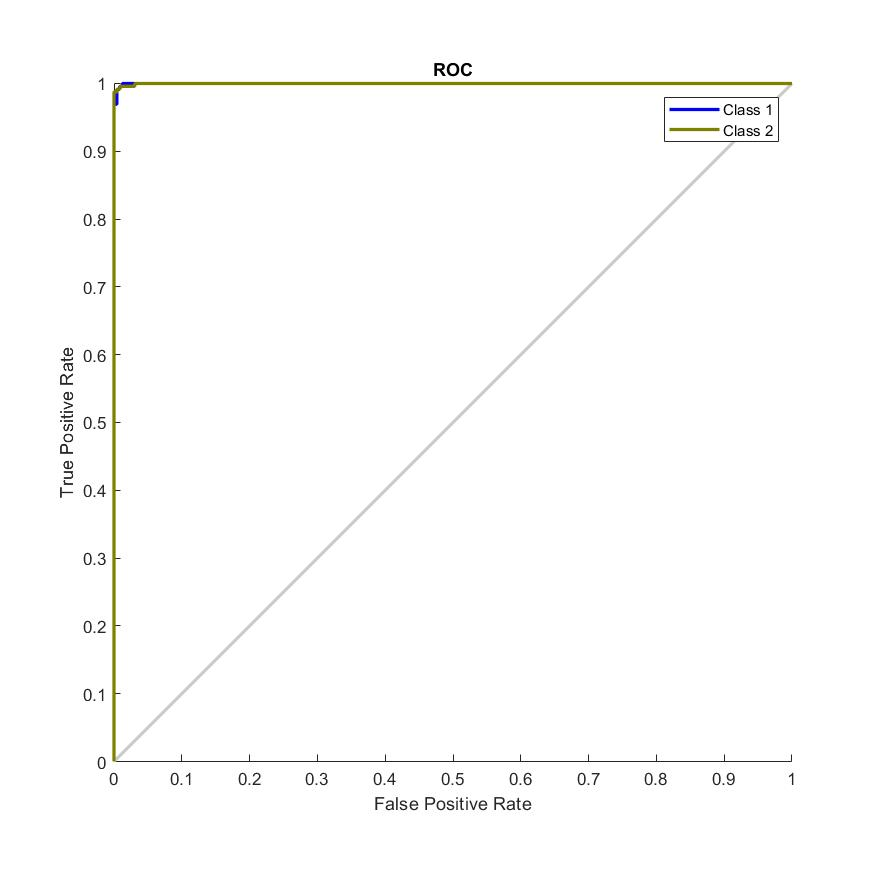
\includegraphics[width=0.8\linewidth]{../images/I_ex4_roc_cancer_dataset_trainbr.jpg}
  \caption{ROC \textit{trainbr}}
 \end{subfigure}
 \begin{subfigure}{0.4\textwidth}
  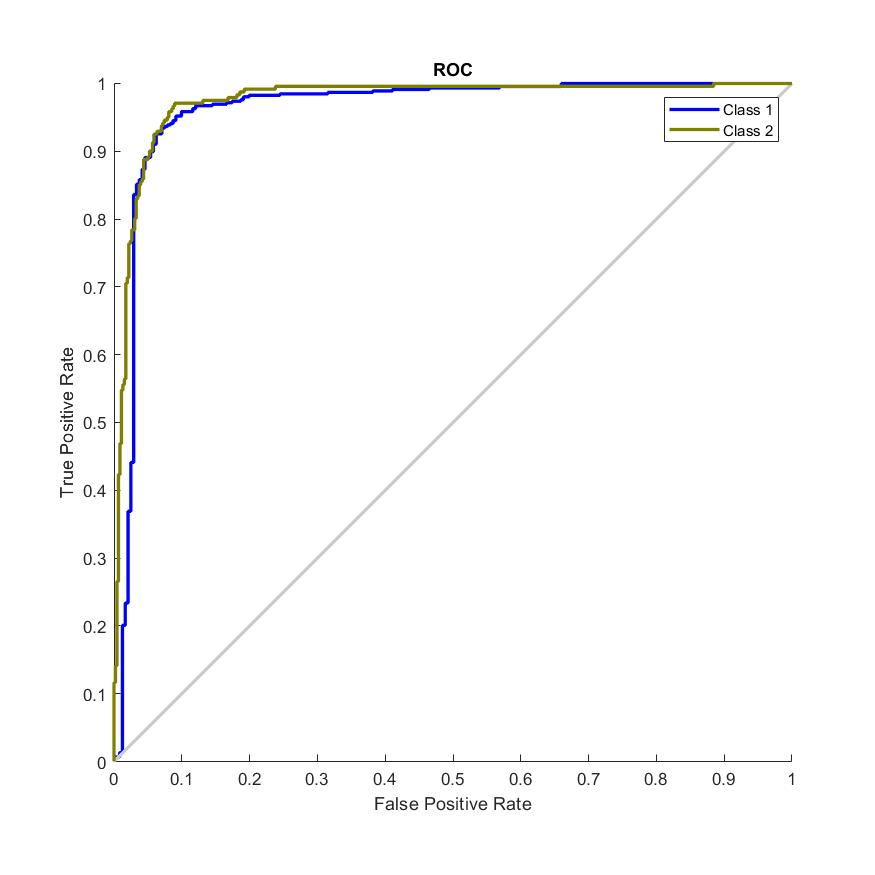
\includegraphics[width=0.8\linewidth]{../images/I_ex4_roc_cancer_dataset_traingd.jpg}
  \caption{ROC \textit{trainrp}}
 \end{subfigure}
 \begin{subfigure}{0.4\textwidth}
  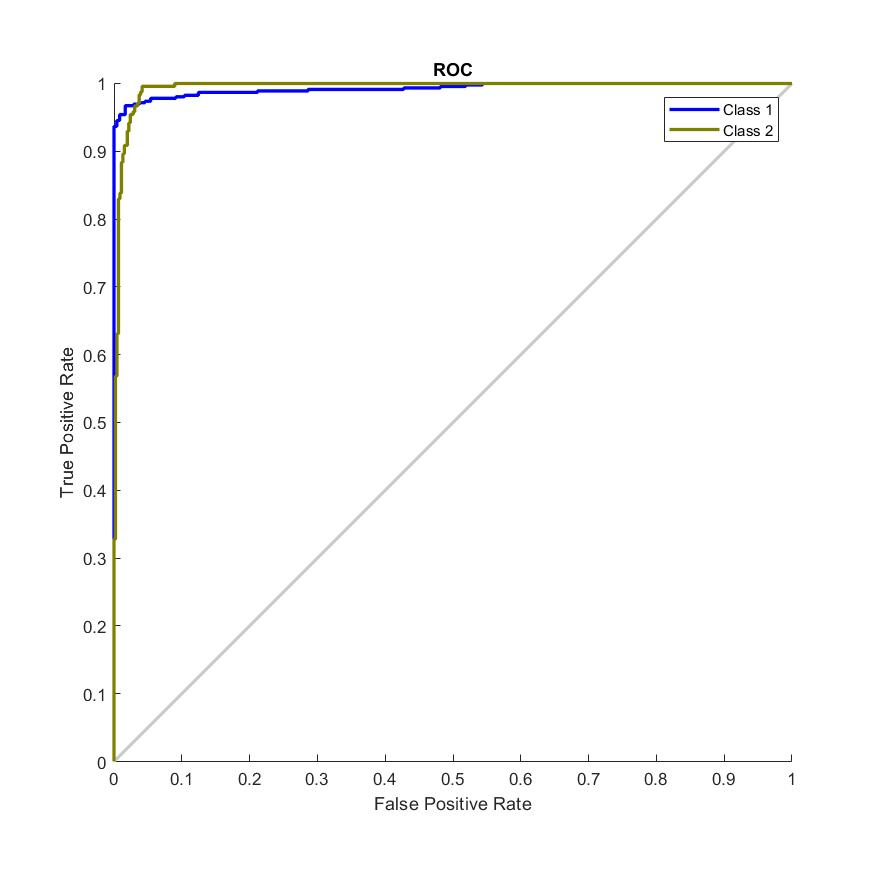
\includegraphics[width=0.8\linewidth]{../images/I_ex4_roc_cancer_dataset_trainoss.jpg}
  \caption{ROC \textit{trainoss}}
 \end{subfigure}
 \begin{subfigure}{0.4\textwidth}
  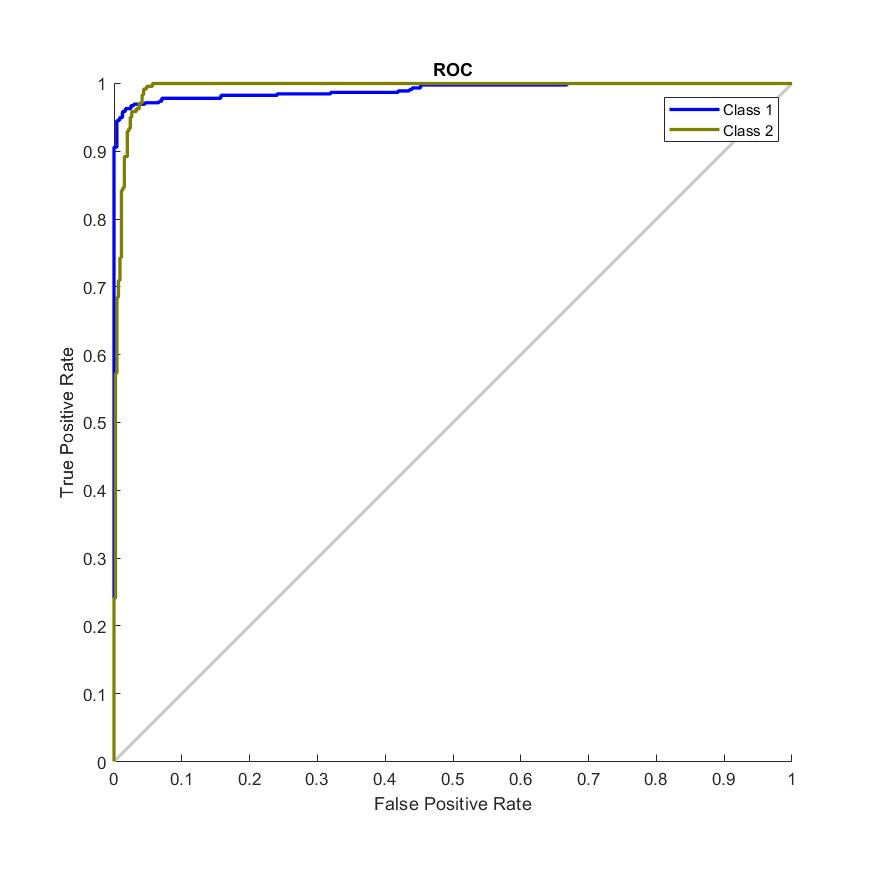
\includegraphics[width=0.8\linewidth]{../images/I_ex4_roc_cancer_dataset_trainrp.jpg}  
  \caption{ROC \textit{traingd}}
 \end{subfigure}
\end{figure}

Evaluando el resultado obtenido de entre las representaciones de \textit{ROC} se
corrobora que el mejor método de entrenamiento pertenece a \textit{trainbr}, y
el peor a \textit{trainrp}; debido a la proximidad/distancia de los valores de
\textit{True Positive Rate} para \textit{False Positive Rate} entre 0 y 0.2.

\end{document}
